\setchapterimage[7.5cm]{images/matt-hardy-6ArTTluciuA-unsplash}
\setchapterpreamble[u]{\margintoc}
\chapter{Basic Concepts of Testing}
\section{Software Quality and Testing}
Software testing is the process of evaluating and verifying that the complete software product or parts of it work and perform as specified by the customer's requirements (SRSD). This process helps in detecting the bugs during the development stage, hence reducing the cost of development and improving performance. In addition, the testing process plays a vital role in achieving and assessing the quality of a software
product \autocite{friedman1995software}. 

Quality assessment activities are discussed in two categories, namely, static analysis and dynamic analysis. Static analysis is based on SRSDs, Software Design Documents (SDD), models, and typically source code. Code review, walkthrough, and inspection are the most common static analysis techniques. The actual execution of the code is not involved in static analysis but rather the source code, byte code, or application binaries are included in the analysis. Static analysis is the more thorough approach and may also prove to be more cost-efficient with the ability to detect bugs at an early phase of the SDLC. Dynamic analysis of a software product involves the actual execution of the code in an attempt to detect bugs. During the dynamic analysis functionality and performance of a program are also observed. Static analysis\index{static analysis} and dynamic analysis\index{dynamic analysis} approaches are complementary to improve the quality of the software product and can be performed in a synchronized and/or planned manner.

In software testing, verification\index{verification} and validation\index{validation} (V\&V) are two similar abstract concepts. Software Engineering standards known as IEEE/ISO/IEC 24765:2017\sidenote{The standard can be found in \url{https://www.iso.org/standard/71952.html}.} (ISO/IEC/IEEE International Standard - Systems and Software Engineering - Vocabulary) defines verification and validation as the process of determining whether the requirements for a system or component are complete and correct, the products of each development phase fulfills the requirements or conditions imposed by the previous phase, and the final system or component complies with specified requirements. In the software world, it is common to define verification process as an answer to the questions, "Are we building the product right?", and validation process as an answer to "Am I building the right product?".

Code reviews\index{code reviews}, inspections\index{inspections}, walkthroughs\index{walkthrough}, and low level tests such as unit testing\index{unit testing}, integration testing\index{integration testing}, static checking\index{static checking} of SRSD and SDD and files are some of the activities for verification, and applying various testing techniques such as acceptance testing, usability testing and other non-functional testing are some of the validation activities. Some of the testing methods such as beta testing, regression testing can be listed as activities at the intersection of V\&V. In this book, the testing activities mentioned here will be explained in detail.

\section{Error, Fault, Defect and Failure}
Error, fault (bug), defect, and failure are very common terms used in software testing. And these terms are sometimes used interchangeably, albeit incorrectly. To avoid confusion and establish their consistent use in software testing area, ISO/IEC/IEEE 24765:2017 “Systems and software engineering — Vocabulary” standard will be used. The definitions taken from this standard and used in this book are given below.

\paragraph{Error}
\index{error}(1) human action that produces an incorrect result, (2) difference between a computed, observed, or measured value or condition and the true, specified, or theoretically correct value or condition, (3) erroneous state of the system.

\paragraph{Fault (bug)}
\index{fault (bug)}(1) manifestation of an error in software, (2) incorrect step, process, or data definition in a computer program, (3) situation that can cause errors to occur in an object, (4) defect in a hardware device or component, (5) defect in a system or a representation of a system that if executed/activated could potentially result in an error.

\paragraph{Defect}
\index{defect}(1) imperfection or deficiency in a work product where that work product does not meet its requirements or specifications and needs to be either repaired or replaced, (2) an imperfection or deficiency in a project component where that component does not meet its requirements or specifications and needs to be either repaired or replaced, (3) generic term that can refer to either a fault (cause) or a failure (effect). 

\paragraph{Failure}
\index{failure}(1) termination of the ability of a system to perform a required function or its inability to perform within previously specified limits; an externally visible deviation from the system's specification.

\section{Objectives of Testing}
The foremost objective of Software Testing is to improve the quality of the product by detecting errors and removing faults made during the development phase of SDLC. 

Providing quality products is the ultimate goal of testing. Customer satisfaction is ensured and as a result, the competitive power of the software company is increased.

In order to comply with these goals, software test teams are established and the product is tested using different methods at each stage (level) of development. These methods of software testing will be elaborated in the chapters that follow.

\section{Test Levels in the V-Model}
Software testing is applied at different levels of development. Considering the so-called V-model\index{V-model}, the levels of testing can be identified as unit (component), integration, system, and acceptance testing. 

While all software development methodologies have different approaches, product development tasks will be performed in the order of (1) requirements gathering and analysis, (2) high-level design, (3) comprehensive design, and (4) coding. 
These tasks match the software testing levels mentioned above as shown in \reffig{fig:v-model}. Unit, Integration and system tests are usually performed by the developers, and acceptance tests by the customer in collaboration with the software developers.

\begin{figure}[!ht]
    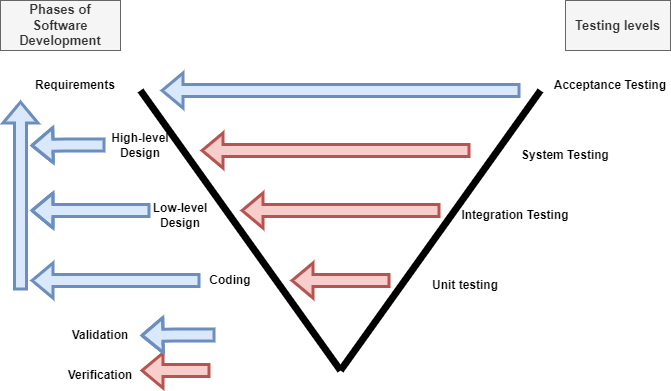
\includegraphics{images/v-model.png}
    \caption{Validation and Verification with the V-model}
    \labfig{fig:v-model}
\end{figure}

In unit testing, individual units/components such as functions, procedures (in developments  with procedural languages) and  methods and classes (in developments with object-oriented languages) are tested. Following the successful completion of the unit tests, related units and components are systematically brought together and subjected to integration tests. The objective of integration testing\index{integration testing} is to build a stable product configuration ready for system tests. 

System level testing\index{system level testing} includes a wide spectrum of testing, such as functionality testing, security testing, robustness testing, load testing, stability testing, stress testing, performance testing, and reliability testing \autocite{naik2011software}. After the successful completion of system level testing, the product is delivered to the customer. The customer performs a series of tests, known as acceptance testing. The main objective of acceptance testing\index{acceptance testing} is to confirm that the system meets the agreed-upon criteria (functional and non-functional requirements), identify and resolve discrepancies, if there are any and determine the readiness of the system for live operations. The final acceptance of a system for deployment is conditioned upon the outcome of the acceptance testing. The acceptance test team produces an acceptance test report which outlines the acceptance conditions. 

Another test level applied at the first three levels is the regression test\index{regression testing}. This test is performed whenever a part of the system (unit, component, or module) is replaced or modified. The main idea of regression testing is to determine if the change creates a side effect (new bugs) on other parts of the software that have already been completed and passed the tests. 

In regression testing, new tests are not designed. Instead, tests are selected, prioritized, and executed from the existing pool of test cases to ensure that nothing is broken in the new version of the software \autocite{naik2011software}. 

\section{White-box and Black-box Testing}
White-box (glass box, clear box, transparent box) testing is a low-level testing technique which deals with the internal working of the software system. During white-box testing, assignment and predicate statements, and the branches and execution paths are considered and checked for possible faults. On the contrary to white-box testing\index{white-box testing}, black-box (data-driven, functional) testing\index{black-box testing} does not care about the internal workings of the code but deals with the overall behaviour and functionality of the parts of a code and as such can be applied at all levels of testing.

White-box testing is suitable at unit and integration levels, whereas black-box testing is ideal at system and acceptance levels. Programming knowledge is necessary for white-box testing. On the contrary, for black-box testing, this is not essential.

\section{Testing Activities}
Main testing activities are planning, analysis, design, implementation, and  execution.  Testing team (or developer) comes up with some requirements to be tested. Test planning considers the team management, cost and the duration of the testing process, and some other related quality assurance metrics. Analysis activity involves understanding the nature of tests to be conducted, complexity of the test, and the risks involved in the execution of the tests. Depending on the tasks to be completed, and the input data required, tests are designed. At the test implementation step tests are chosen and prioritized. Software test execution is the last activity to perform. Test results are systematically collected and reported along with the required testing metrics.

A test plan can have more than one test suite. Each test suite has one or more related test cases. A test case (TC) is usually\index{test suite} defined as a pair of \textbf{<input, expected outcome>}. If a code\index{test case} under test is to compute the absolute value of a real number, say, x, then one can list three test cases as follows:
\begin{itemize}[nosep]
    \item TC1: <0.0, 0.0>
    \item TC2: <-26.4, +26.4>
    \item TC3: <+14.0, +14.0>
\end{itemize}
A test case is prepared using the requirements and functional specifications, source code, and input/output domains. Expected outcome can be as simple as a single numerical value, a more complex data type like audio, photo or video, a state change or a set of values which needs to be interpreted together for the outcome to be valid \autocite{naik2011software}.

Another important concept in testing is test oracle. A test oracle\index{test oracle} (or simply oracle) is a mechanism for determining whether a test has passed or failed. An oracle will respond with a pass or a fail verdict on the acceptability of any test sequence for which it is defined. When executing a test case, the correctness of the implementation is confirmed by an oracle.

In most testing environments, test oracle is the human who designs the test \autocite{bertolino1996use}. A simple example of a test oracle is given below\sidenote{Detailed information about test oracle can be found in the link: \url{https://bit.ly/3K9iqZj}}. 

Given a list of 3 integers, 11, 23, and 19, what is the expected value from a function, say, computeMax(), which returns the maximum? In this case, the test oracle is easy to identify.

\begin{itemize}
    \item \lstinline!int expected = 23!; 
    \item \lstinline!int actual = computeMax(11, 23, 19);! \lstinline!computeMax! is a method which returns the maximum of the three numbers.
    \item \lstinline!assertEquals(expected, actual);!
\end{itemize}

Note that \lstinline!assertEquals()!\index{assertEquals()} is a method in the JUnit testing library to compare two objects for equality. This method will be introduced during laboratory sessions.

\section{Problems}
\begin{enumerate}
    \item Create test cases for a computer program to find the positive square root of a real number.
    \item Discuss the difference between white-box and black-box testing strategies.
    \item What is a stateless software system? Give an example.
    \item ATM is an example of a state-oriented system. Create a test case for withdrawing money from a bank account. First define the input, and write down the expected output(s) during the transaction.\\
    \emph{Hint. In this case, a test case will contain more than one <input, expected> pairs and input may be choosing an item from a menu.}
    \item What is agile software testing? 
    \item What are the main differences between classical testing and agile testing approaches?
    \item What is Test Driven Development (TDD)?
    \item What is a test oracle? Explain by using a simple testing activity.
    \item Differentiate between verification and validation. Describe various verification and validation methods.
    \item What is the main difference between inspections and walkthroughs?
\end{enumerate}